\documentclass[]{article}

%opening
\title{4F13 Probabilistic Machine Learning - Latent Dirichlet Allocation}
\author{Candidate: 5562E}

%packages
\usepackage[margin=0.5in]{geometry}
\usepackage[export]{adjustbox}
\usepackage{mathtools}
\usepackage{graphicx}
\usepackage{amsmath}
\usepackage{amssymb}
\usepackage{hyperref}
\usepackage{caption}
\usepackage{subcaption}
\usepackage{parskip}
\usepackage{listings}
\usepackage{pdfpages}
\usepackage{bbm}

%package setup
\graphicspath{{./img/}}
\DeclareMathOperator*{\argmax}{arg\,max}
\DeclareMathOperator*{\argmin}{arg\,min}

%custom commands
\newcommand{\Fcal}{\mathcal{F}}
\newcommand{\idft}{\mathcal{F}^{-1}}
\newcommand{\Xcal}{\mathcal{X}}
\newcommand{\Ncal}{\mathcal{N}}
\newcommand{\Acal}{\mathcal{A}}
\newcommand{\Bcal}{\mathcal{B}}
\newcommand{\cmplx}{\mathbb{C}}
\newcommand{\Lcal}{\mathcal{L}}
\newcommand{\Mcal}{\mathcal{M}}
\newcommand{\indep}{\perp \!\!\! \perp}
\newcommand{\iid}{\stackrel{iid}{\sim}}
\newcommand{\figwidth}{0.6\linewidth}
\newcommand{\betaml}{\hat{\beta}^{ML}}
\newcommand{\Expect}{\mathbb{E}}


%section numbering
\renewcommand{\thesubsection}{\alph{subsection}}

\begin{document}

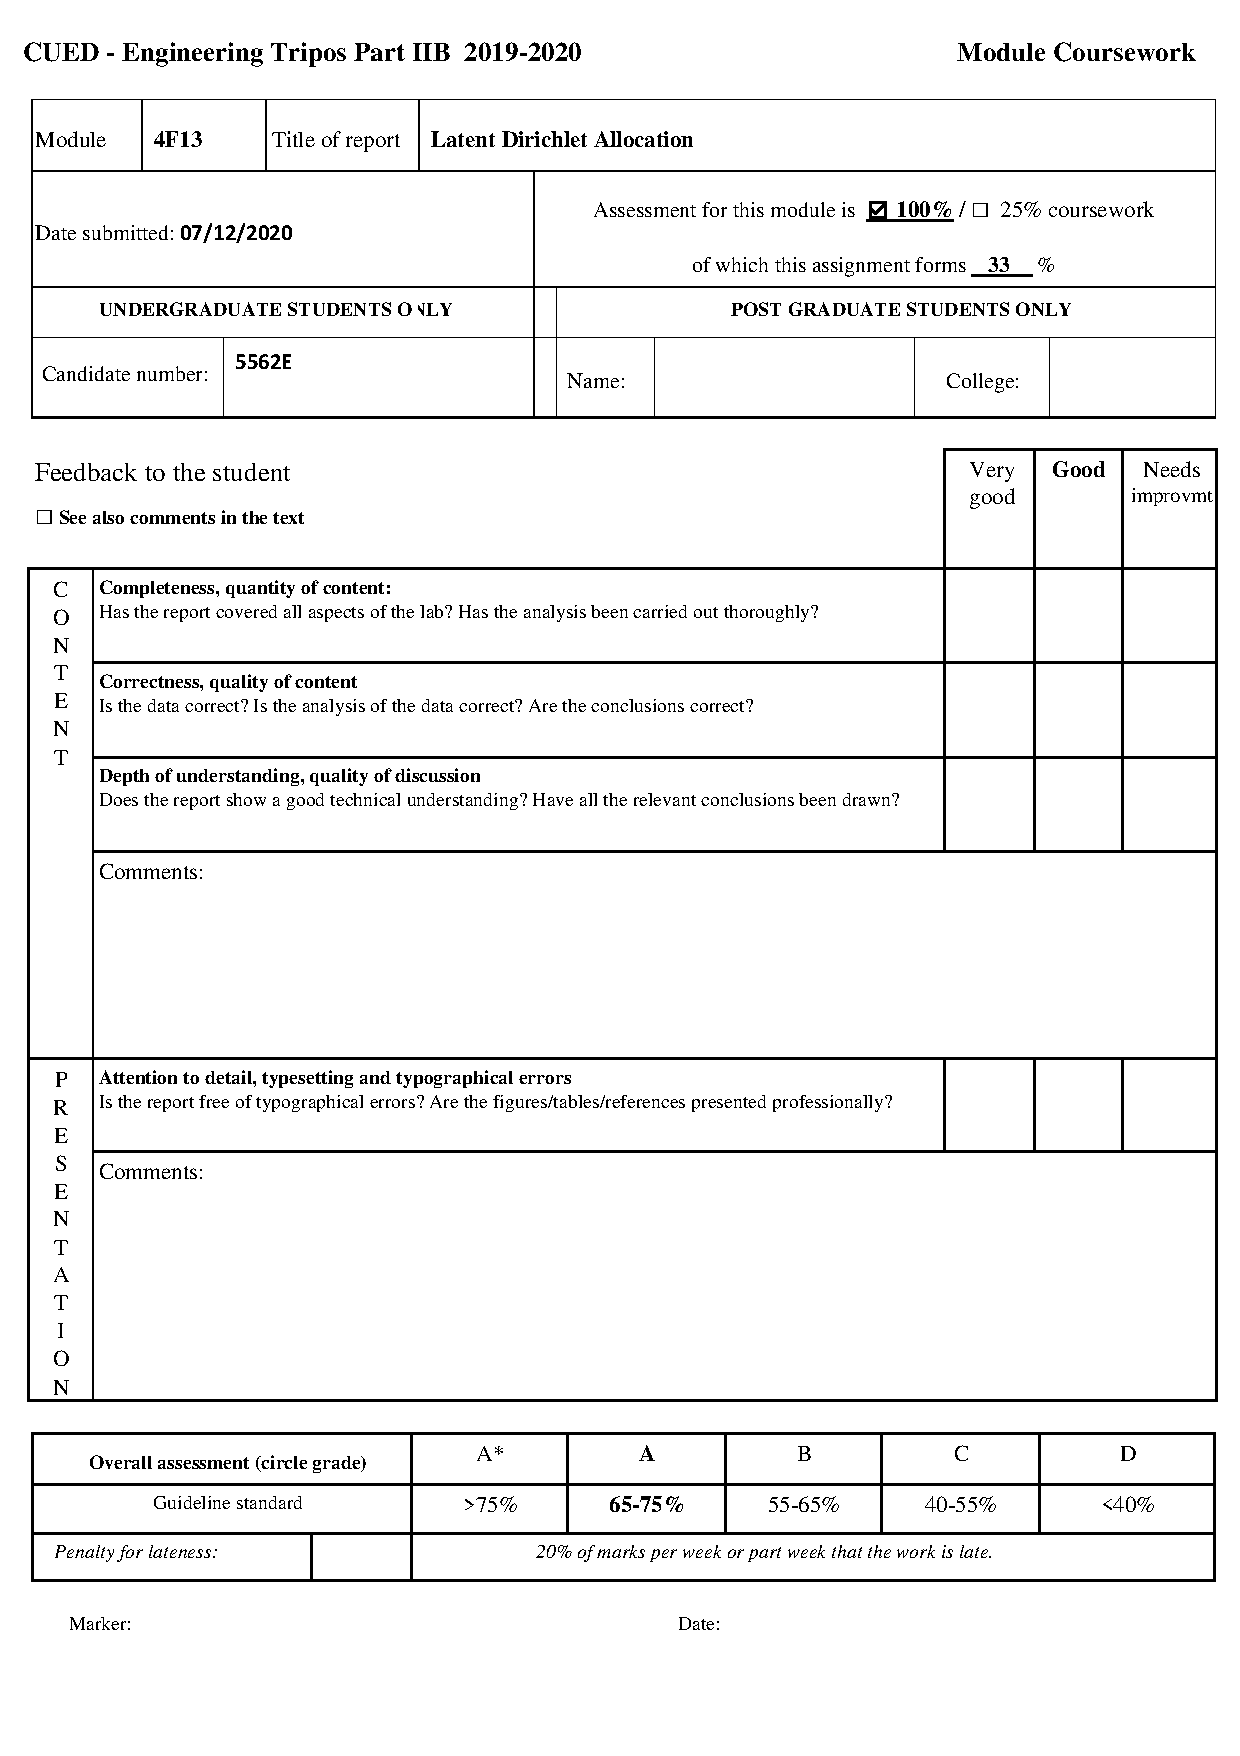
\includepdf[pages={1}]{coversheet-CW3.pdf}

\setcounter{page}{1}
\maketitle

\tableofcontents

\section{Introduction}

We have a document test set $\Acal$, which consists of $D$ documents indexed by $d \in \{1 \dots D\}$. A document is an ordered list of words. The vocabulary $\Mcal$ has $M=|\Mcal|$ unique words. We denote the $n$'th word in the $d$'th document by $w_{nd} \in \{1 \dots N_d\}$. Where $N_d$ is the length of document $d$. For simplicity we denote the count of occurrences of word $m$ in the test set by $c_m$.

We hold back a test set $\Bcal$ to calculate the performance of our approaches.

\section{Questions}
\subsection{Maximum Likelihood}

We begin by assuming that each word is drawn independently from a categorical distribution with parameter $\beta$: $w_{nd} \iid Cat(\beta)$. In this case $\beta$ is a $M \times 1$ vector with the conditions that $\sum_{m=1}^{M} \beta_m = 1$ and $\beta_i \geq 0$. The likelihood of the parameter $\beta$ is the probability of the dataset given $\beta$:
%
\begin{equation}
	L(\beta) = P(\Acal | \beta) = \prod_{d=1}^{D} \prod_{n=1}^{N_d} P(w_{nd} | \beta) = \prod_{m \in \Mcal} \beta_m ^{c_m}
\end{equation}
%
Where $c_m$ is the count of word $m$ in the training set. We wish to obtain the Maximum-Likelihood estimate $\betaml = \argmax L(\beta)$. We prefer to maximise the log-likelihood as this is more tractable:
%
\begin{equation}
	\Lcal(\beta) = \log L(\beta) = \sum_{m \in \Mcal} c_m \log \beta_m
\end{equation}
%
We can now take derivatives and include a Lagrange multiplier to respect the sum to 1 constraint:
%
\begin{equation*}
	\frac{\partial}{\partial \beta_i}  \left\{ \Lcal(\beta) + \lambda \left(1 - \sum_{m=1}^{M} \beta_m \right) \right\}_{\beta = \betaml} = \frac{c_i}{\betaml_i} - \lambda= 0
\end{equation*}
\begin{equation}
	\therefore \betaml_i = \frac{c_i}{\lambda} = \frac{c_i}{\sum_{m \in \Mcal} c_m} = \frac{c_i}{C}
\end{equation}
%
Therefore, the ML estimate is simply the empirical frequency of each word (normalised by the sum of all counts $C$). For the training set $\Acal$ we have $C_\Acal = 271898$.
%
\begin{figure}[!h]
	\begin{subfigure}{0.5\linewidth}
		\centering
		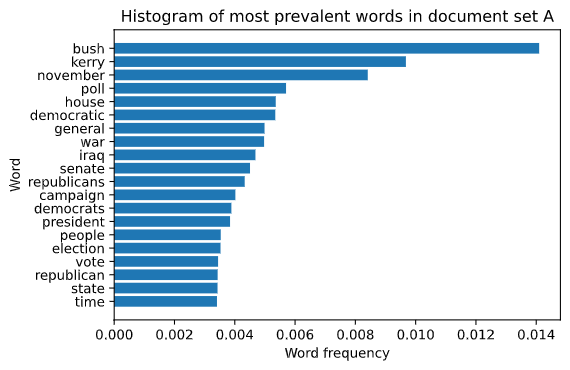
\includegraphics[width=\linewidth]{hist-ml.png}
		\caption{Top 20 most prevalent words}
		\label{fig:hist-ml-max}
	\end{subfigure}
	\begin{subfigure}{0.5\linewidth}
		\centering
		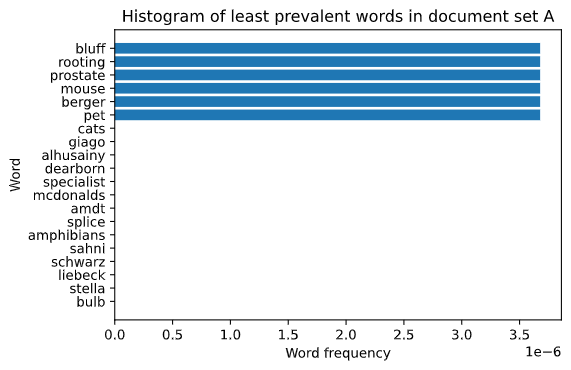
\includegraphics[width=\linewidth]{hist-ml-min.png}
		\caption{Top 20 least prevalent words}
		\label{fig:hist-ml-min}
	\end{subfigure}
	\caption{ML estimate of word probabilities trained on set $\Acal$}
	\label{fig:hist-ml}
\end{figure}
%
Figure \ref{fig:hist-ml-max} shows the empirical frequencies of the top 20 words in document set $\Acal$. We have that $\betaml_{\max} \coloneqq \frac{\max_i c_i}{C} = \frac{3833}{271898}$ for the word \textit{``bush''} (the president - not the foliage). Likewise $\betaml_{\min} \coloneqq \frac{\min c_i}{C} = 0$ as there are some words in the vocabulary $\Mcal$ that never appear in the training set $\Acal$ (such as \textit{``bulb''} in \ref{fig:hist-ml-min}). Indeed, each new word $w^*$ under ML is assumed to be drawn from:
%
\begin{equation}
	P(w^* = i | \betaml) = \frac{c_i}{C}
	\label{eqn:ml-est}
\end{equation}
%
Therefore, if we have an arbitrary test set $\mathcal{T}$ that is $T$ words long. The maximum probability test set would be $T$ repetitions of \textit{``bush''}. The lowest probability test set need only have a single word with zero probability under our ML estimate (e.g. \textit{``bulb''}) to make the probability of the whole multiply to 0.
%
\begin{align}
	\log P(\mathcal{T}) |_{\max} &= T \log \betaml_{\max} = \frac{3833}{271898} T \\
	\log P(\mathcal{T}) |_{\min} &=  0
\end{align}
%
This is clearly unsatisfactory; a feasible test set should not have zero probability. Therefore, the ML estimate is insufficient.
 
\subsection{Bayesian Inference}

Instead, we can perform Bayesian inference to ameliorate these issues. We assume the probability vector $\beta$ has a Dirichlet prior $\beta \sim Dir(\beta ; \alpha)$ with concentration parameter $\alpha$ - where $\alpha$ and $\beta$ are the same shape. We perform Bayesian inference to obtain the posterior for $\beta$.
%
\begin{align}
	P(\beta | \Acal) &\propto P(\beta) \cdot P(\Acal | \beta) \nonumber \\
	&= \left( \frac{1}{B(\alpha)} \prod_{m = 1}^{M} \beta_m^{\alpha_m -1} \right) \cdot \prod_{p=1}^{M} \beta_m^{c_m} \nonumber \\
	&\propto \prod_{m = 1}^{M} \beta_m^{(\alpha_m + c_m) -1} \nonumber \\
	&\propto Dir(\beta ; \alpha + c) \nonumber \\
	\therefore P(\beta | \Acal) &= Dir(\beta ; \alpha + c)
	\label{eqn:posterior}
\end{align}
%
Where, $c$ is now a vector of word counts. We say that the Dirichlet distribution is a conjugate prior to the categorical / multinomial distribution because the posterior is also Dirichlet (albeit with a new parameter). We now seek to compute the predictive distribution for a new word $w^*$ given the posterior.
%
\begin{align}
\begin{split}
	P(w^* = i | \Acal) &= \int_{\beta} P(w^* = i, \beta | \Acal) d\beta \\
	&= \int_{\beta_i} P(w^* = i | \beta , \Acal) \int_{\beta_{\backslash i}} P(\beta | \Acal) d\beta_{\backslash i} d\beta_i \\
	&= \int P(w^* = i | \beta_i) P(\beta_i | \Acal) d\beta_i \\
	&= \int \beta_i P(\beta_i | \Acal) d\beta_i \\
	&= \Expect_{\beta_i | \Acal} [\beta_i] \\
	&= \frac{\alpha_i + c_i}{\sum_{m=1}^{M} \alpha_m + c_m} \coloneqq \hat{\beta}^*_i
\end{split}
\end{align}
%
Where the last line is a simple property of the Dirichlet: the mean of each component is proportional to the corresponding parameter value (subject to normalisation). An interesting observation is that the predictive distribution is exactly equal to that computed using the MAP estimate ($\hat{\beta}^* = \hat{\beta}^{MAP}$). If we consider only a symmetric Dirichlet such that $\alpha = a \mathbf{1}$. The previous expression reduces to:
%
\begin{equation}
	P(w^* = i | \Acal) = \frac{a + c_i}{Ma + C}
	\label{eqn:pred-bayes}
\end{equation}
%
By comparing equations \ref{eqn:ml-est} and \ref{eqn:pred-bayes}, we see that the posterior has the effect of adding a pseudo-count $a$ to each word prior to observing the training set $\Acal$.
%
\begin{align}
\begin{split}
	P(w^*=i | \Acal) &> P(w^*=i | \betaml) \\
	\frac{a + c_i}{Ma + C} &> \frac{c_i}{C} \\
	Ca + Cc_i &> Mac_i + Cc_i \\
	c_i &< \frac{C}{M}
\end{split}
\end{align}
%
As the prior is symmetric the same pseudo-count $a$ is added to each word. Those with $c_i < C/M$ gain probability and those with $c_i > C/M$ lose it. The effect is that all word probabilities are drawn closer to $C/M$ but importantly no probability rank orderings stay the same. The larger the value of $a$, the stronger this effect and the less importance is assigned to the frequency observations in $\Acal$.

\subsection{Testing Performance}

We now apply this Bayesian analysis to an unseen test document. The log probability of all words in a document $d$ is denoted by $\{w^*_{nd}\}_{n=1}^{N_d}$. To compute the log probability $l(d)$:
%
\begin{align}
\begin{split}
	l(d) &\coloneqq \log P(\{w^*_{nd}\}_{n=1}^{N_d} | \Acal) \\
	&= \log \prod_{n=1}^{N_d} P(w^*_{nd} | \Acal) \\
	&= \log \prod_{m = 1}^{M} P(w^*=m | \Acal)^{c^*_{md}} \\
	&= \sum_{m=1}^{M} c^*_{md} \log P(w^* = m | \Acal) \\
	&= \sum_{m=1}^{M} c^*_{md} \log \frac{a+c_m}{Ma+C} \\
	&= (c^*_d)^T \log \hat{\beta}^{*}
\end{split}
\label{eqn:test-doc-prob}
\end{align}
%
Where $c^*_{md}$ is the count of word $m$ in the unseen document $d$. All words are independent, hence how we can factorise the first line. Word order matters. Therefore, we treat a document as a sequence of categorical r.v.'s rather than a single multinomial over word counts; we omit a combinatoric term for all the various permutations of words in a document. The phrase \textit{``Bush beats Kerry''} is very different to \textit{``Kerry beats Bush''} so we treat each phrase as a separate document rather than combining their probabilities.

 We set the pseudo-count parameter to $a=10$ and apply equation \ref{eqn:test-doc-prob} to test document $d=2001$, to obtain:
 %
 \begin{equation}
 	l(d=2001)|_{a=10} = -3682.3
 \end{equation}
 %
 As well as the log probability of document $d$, we are interested in the per-word perplexity $p(d)$ defined in equation \ref{eqn:perplex}.
%
\begin{equation}
p(d) \coloneqq \exp \left(- \frac{l(d)}{N_d} \right)
\label{eqn:perplex}
\end{equation}
%
The expected perplexity of rolls from an $n$-sided die is $n$ and so the expected perplexity for samples drawn from a uniform multinomial with $M$ total categories would be $M$. This is the maximum perplexity of a multinomial with $M$ categories as we have maximum uncertainty. We can compute the perplexities for a single document or for all documents by simply concatenating documents after one another. The results are given in table \ref{tab:perplex}.
%
\begin{table}[!h]
	\centering
	\begin{tabular}{c | c c c}
		& One doc $d=2001 \in \Bcal$ & All docs $\forall d \in \Bcal$ & Uniform multinomial \\ \hline
		per-word perplexity & 4310.8 & 2687.1 & $M=6906$
	\end{tabular}
\caption{Perplexities of documents in test set $\Bcal$}
\label{tab:perplex}
\end{table}
%
Documents with a higher prevalence of common words have higher log-probability and hence lower perplexity. Indeed document $d=2001$ has a higher perplexity than the average in set $\Bcal$ so we conclude that this document contain rarer words than in the rest of the set.

\textbf{Words}: XX

\end{document}
